\documentclass{beamer}
\usepackage{tabularx}
\usepackage{graphicx}
\usepackage{multimedia}
%Information to be included in the title page:
\title{Design specification \newline AquaElevate}
\subtitle{Dead fish handling}
%\author{Anonymous}
\institute{Operational systems - ScaleAQ}
\date{\today}

\begin{document}

\frame{\titlepage}

\begin{frame}
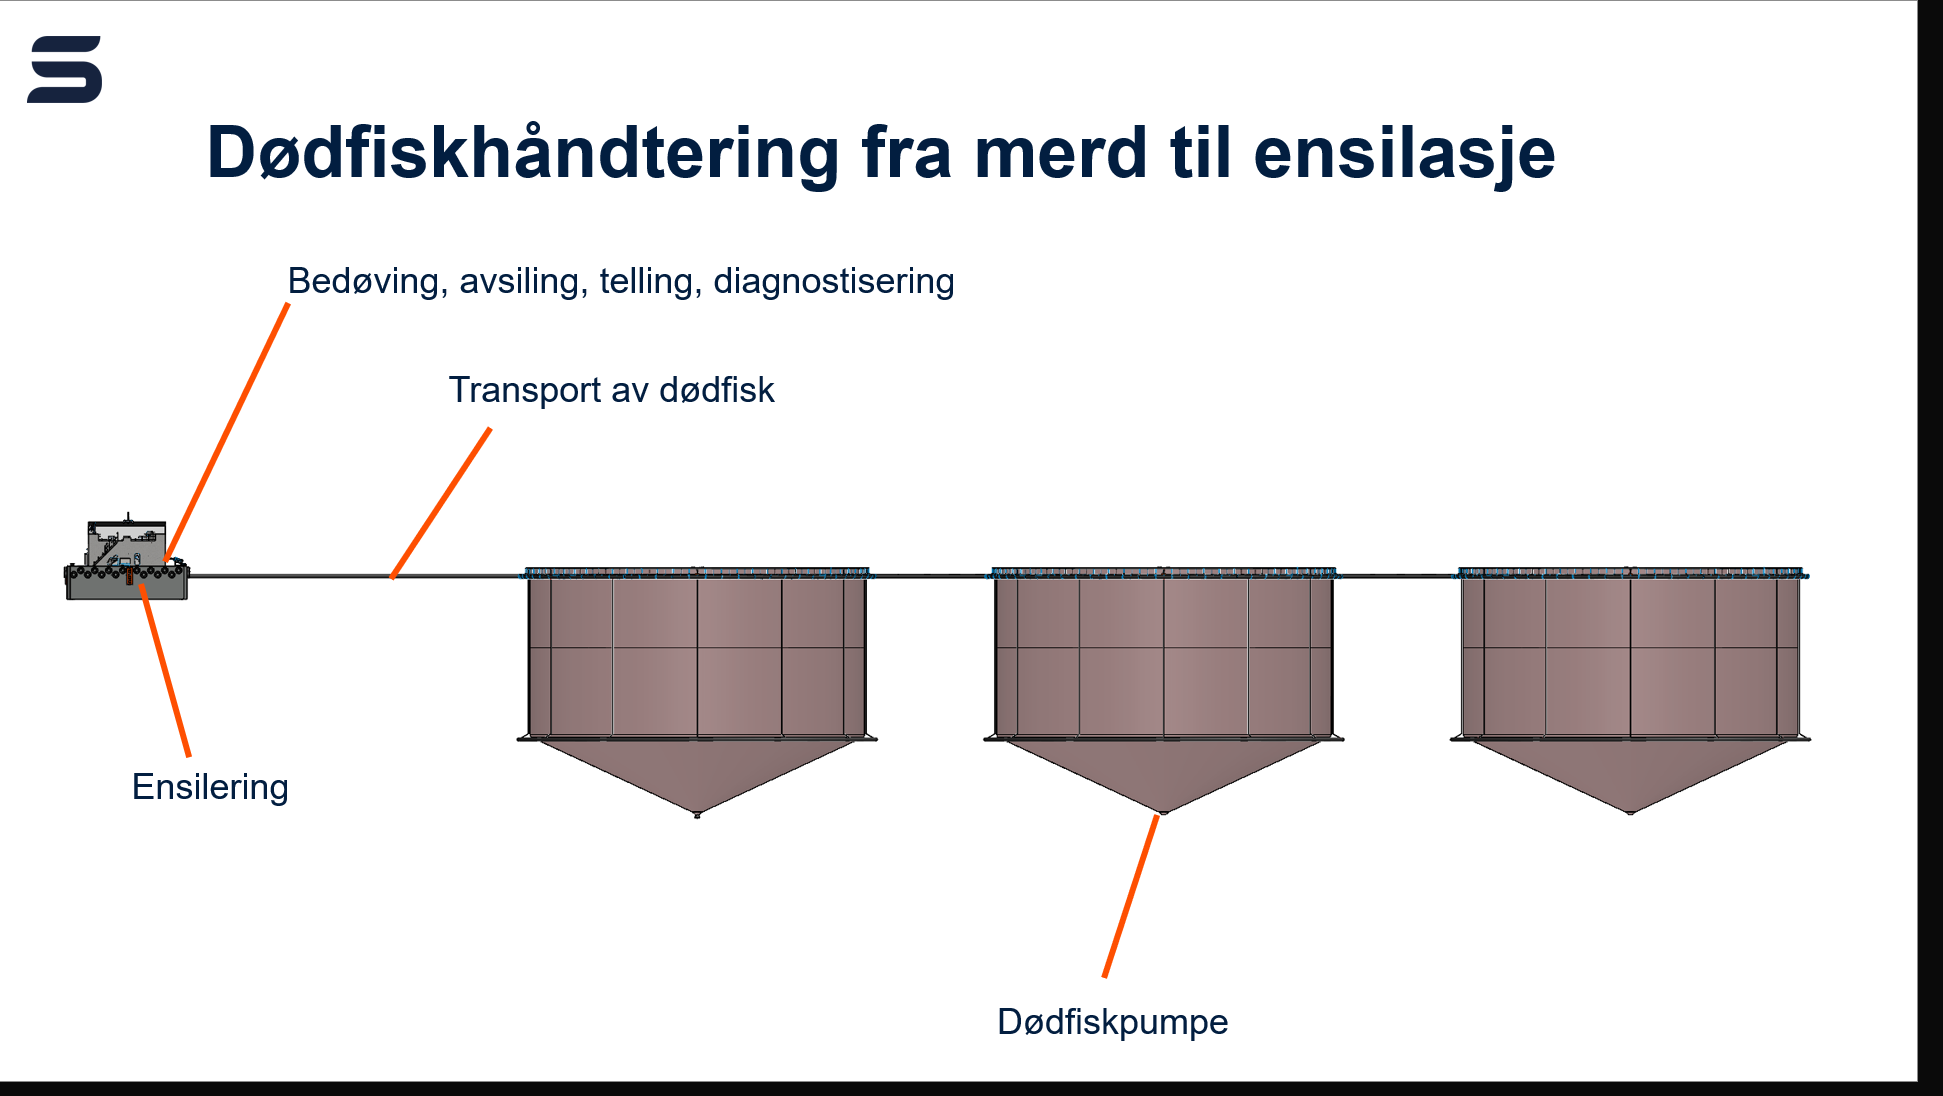
\includegraphics[width=\textwidth]{overview.png}
\end{frame}

\begin{frame}
  \frametitle{System overview}
\begin{minipage}[t]{0.5\textwidth}
\scriptsize 
    \begin{enumerate}
    \vspace{0pt} % <-- forces top alignment inside the minipage
    \item<1-> Dead fish are gathered at the bottom of the pen.
    \item<2-> The fish flows through a GRP pipe from the pen and up to the LiftUp unit.
    \item<3-> Stunner unit (state mandatory)
    \item<4-> It then moves through the liftup-unit by means of gravity and a VSD controlled conveyor belt
    \item<5-> Flushing system
    \item<6-> Camera unit / vision system
    \item <7-> Distance sensor
    \item <8-> Moves through a pre-grinder
    \item <9-> Stored in tanks and continuously circulated/grinded in the ensilage system.
    \item <10-> Automatic handling of acid dosing
    \end{enumerate}
\end{minipage}%
\hfill%
\begin{minipage}[t]{0.5\textwidth}
    \vspace{0pt} % top alignment for images
    \includegraphics<1>[width=0.8\textwidth]{deadfishpen.png}
    \includegraphics<2>[width=0.7\textwidth]{airliftpumppres.png}
    \includegraphics<3>[width=0.8\textwidth]{liftup2.jpg}
    \includegraphics<4-6>[width=0.8\textwidth]{liftupmodel.png}
    \includegraphics<7>[width=0.8\textwidth]{fishpresent.png}
    %
    \includegraphics<7>[width=0.8\textwidth]{sick.png}
    \includegraphics<8>[width=0.8\textwidth]{pregrinder.png}
    \includegraphics<9-10>[width=0.8\textwidth]{ensilage.png}

\end{minipage}

\end{frame}


\begin{frame}
  \frametitle{Compressor}
  \begin{minipage}[t]{0.5\textwidth}
\scriptsize 
    \begin{enumerate}
    \vspace{0pt} % <-- forces top alignment inside the minipage
    \item<1-> Will be continuously running in subsea applications. Will only run when dead fish system is active on other pens.
    \item<2-> Responsibilities are delivering air to
    \begin{itemize}
      \item<3-> {\footnotesize a buffer tank used for refilling the air domes in the susbea pens}.
      \item<4-> {\footnotesize the air pump at the bottom of the pens for collecting dead fish.}
    \end{itemize}
    \item<5-> Controlled and monitored in the PLC by hardwired (+24VDC) signals.
    \item Has its own local user interface with configuration and setting possibilities.
    \end{enumerate}
\end{minipage}%
\hfill%
\begin{minipage}[t]{0.5\textwidth}
    \vspace{0pt} % top alignment for images
    \includegraphics<1->[width=0.8\textwidth]{ga30vsd.png}
\end{minipage}
\end{frame}

\begin{frame}
  \frametitle{LiftUp unit}
  \begin{minipage}[t]{0.5\textwidth}
\scriptsize 
    \begin{enumerate}
    \vspace{0pt} % <-- forces top alignment inside the minipage
    \item<1-> Consists of different subsystems.
    \begin{itemize}
    \item<2-> Stunner
    \item<3-> Flusher
    \item<4-> Pen selector control
    \item<5-> Conveyor belt
    \item<6-> Camera diagnostic unit
    \end{itemize}
    \item<7-> All components connected to Framo's local PLC on the unit.
    \item<8-> Modbus TCP/IP interface to the local PLC for monitoring and control.
    \item<9-> Local user interfcace
    \end{enumerate}
\end{minipage}%
\hfill%
\begin{minipage}[t]{0.5\textwidth}
    \vspace{0pt} % top alignment for images
    \includegraphics<1-8>[width=0.8\textwidth]{liftup3.jpg}
    \includegraphics<9>[width=1.2\textwidth]{liftupUI.png}
\end{minipage}
\end{frame}

\begin{frame}
  \frametitle{Ensilage unit}
  \begin{minipage}[t]{0.5\textwidth}
\scriptsize 
    \begin{enumerate}
    \vspace{0pt} % <-- forces top alignment inside the minipage
    \item<1-> Consists of different subsystems.
    \end{enumerate}
\end{minipage}%
\hfill%
\begin{minipage}[t]{0.5\textwidth}
    \vspace{0pt} % top alignment for images
    \includegraphics<1-8>[width=0.8\textwidth]{liftup3.jpg}
\end{minipage}
\end{frame}


\begin{frame}
\frametitle{Scenarios}
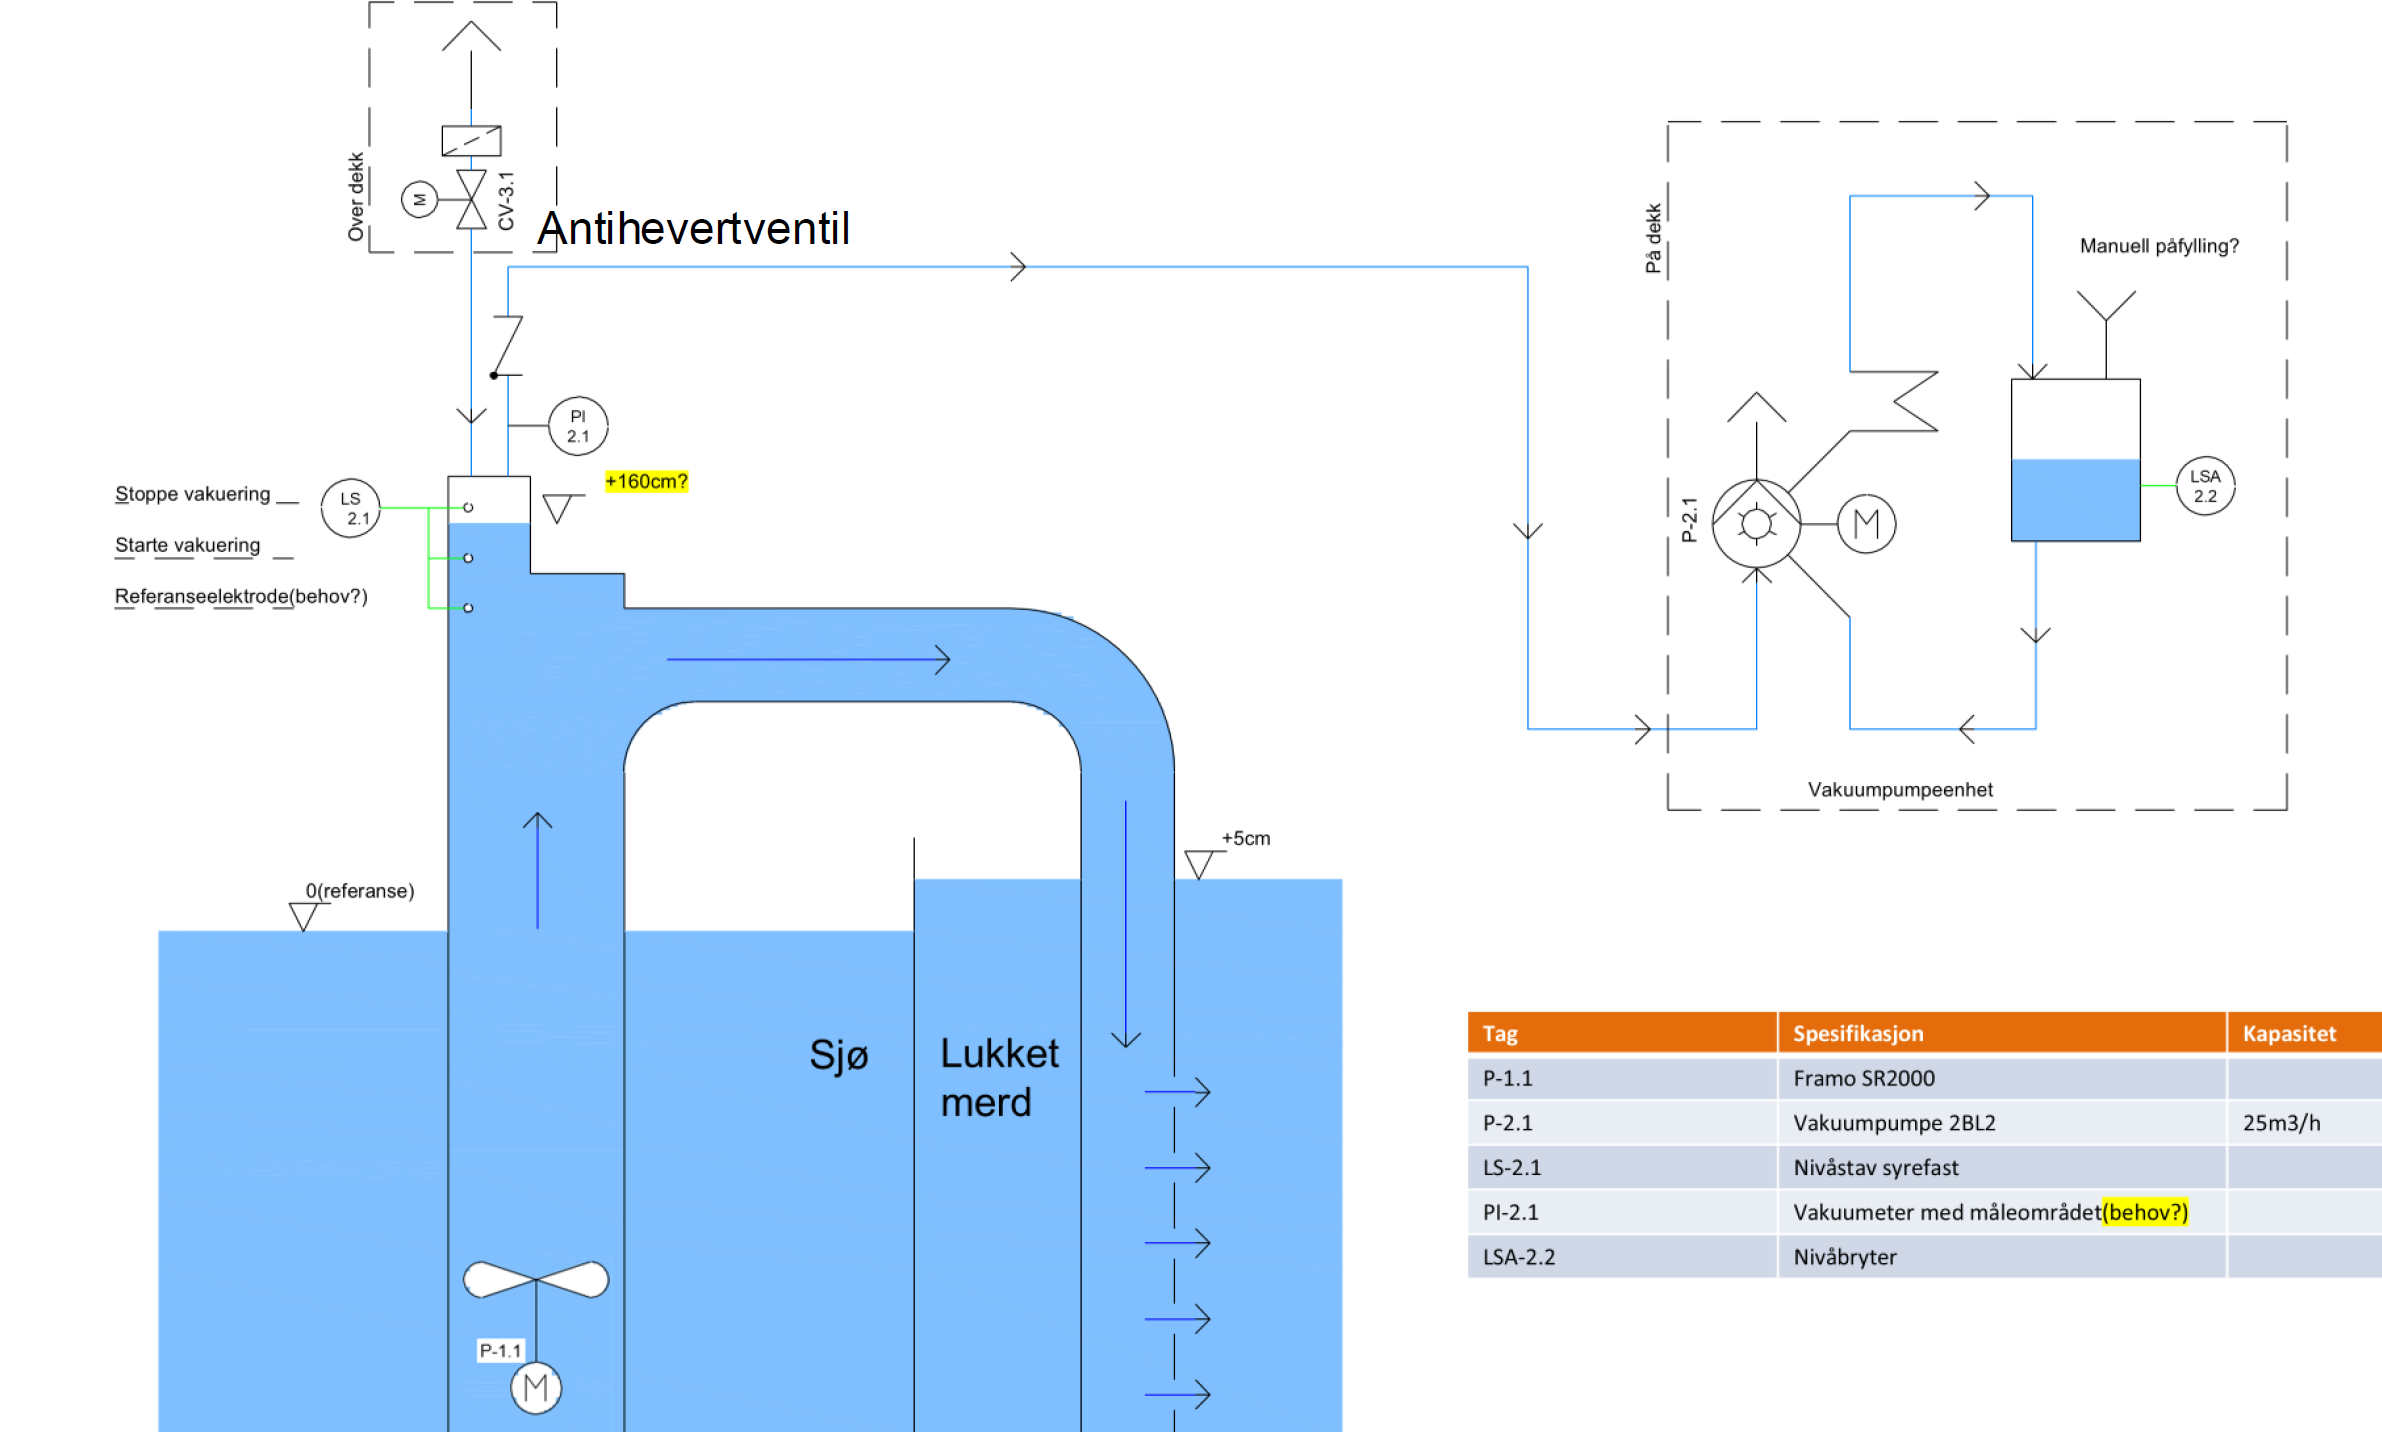
\includegraphics [width=.53\textwidth]{siphon.png} \newline
\framebox{\parbox{\dimexpr\linewidth-2\fboxsep-2\fboxrule}{
\scriptsize \begin{enumerate}
\item<1-> All systems are powered up and outlet valve is in position within valid range.
\item<2-> User sends start command to pump no. 1
\item<3-> System checks condition of process and begins the starting sequence of inlet pump.
\item<4-> The pumps starts at reduced speed, vacuum system starts and anti-siphon valve closes.
\item<5-> After a limit switch at outlet piping triggers, the vacuum pump stops and the pump starts running at reduced speed
\item<6-> System changes to "remote operation" and in "manual mode" at 50 RPM.
\end{enumerate}
\textbf{Finish}
\vspace{0.1cm}
\hrule
\vspace{0.1cm}
Scenario 1 - Cold start of inlet pump no. 1 into manual operation mode at a given speed.
  }}


\end{frame}

\begin{frame}
\frametitle{Scenarios}
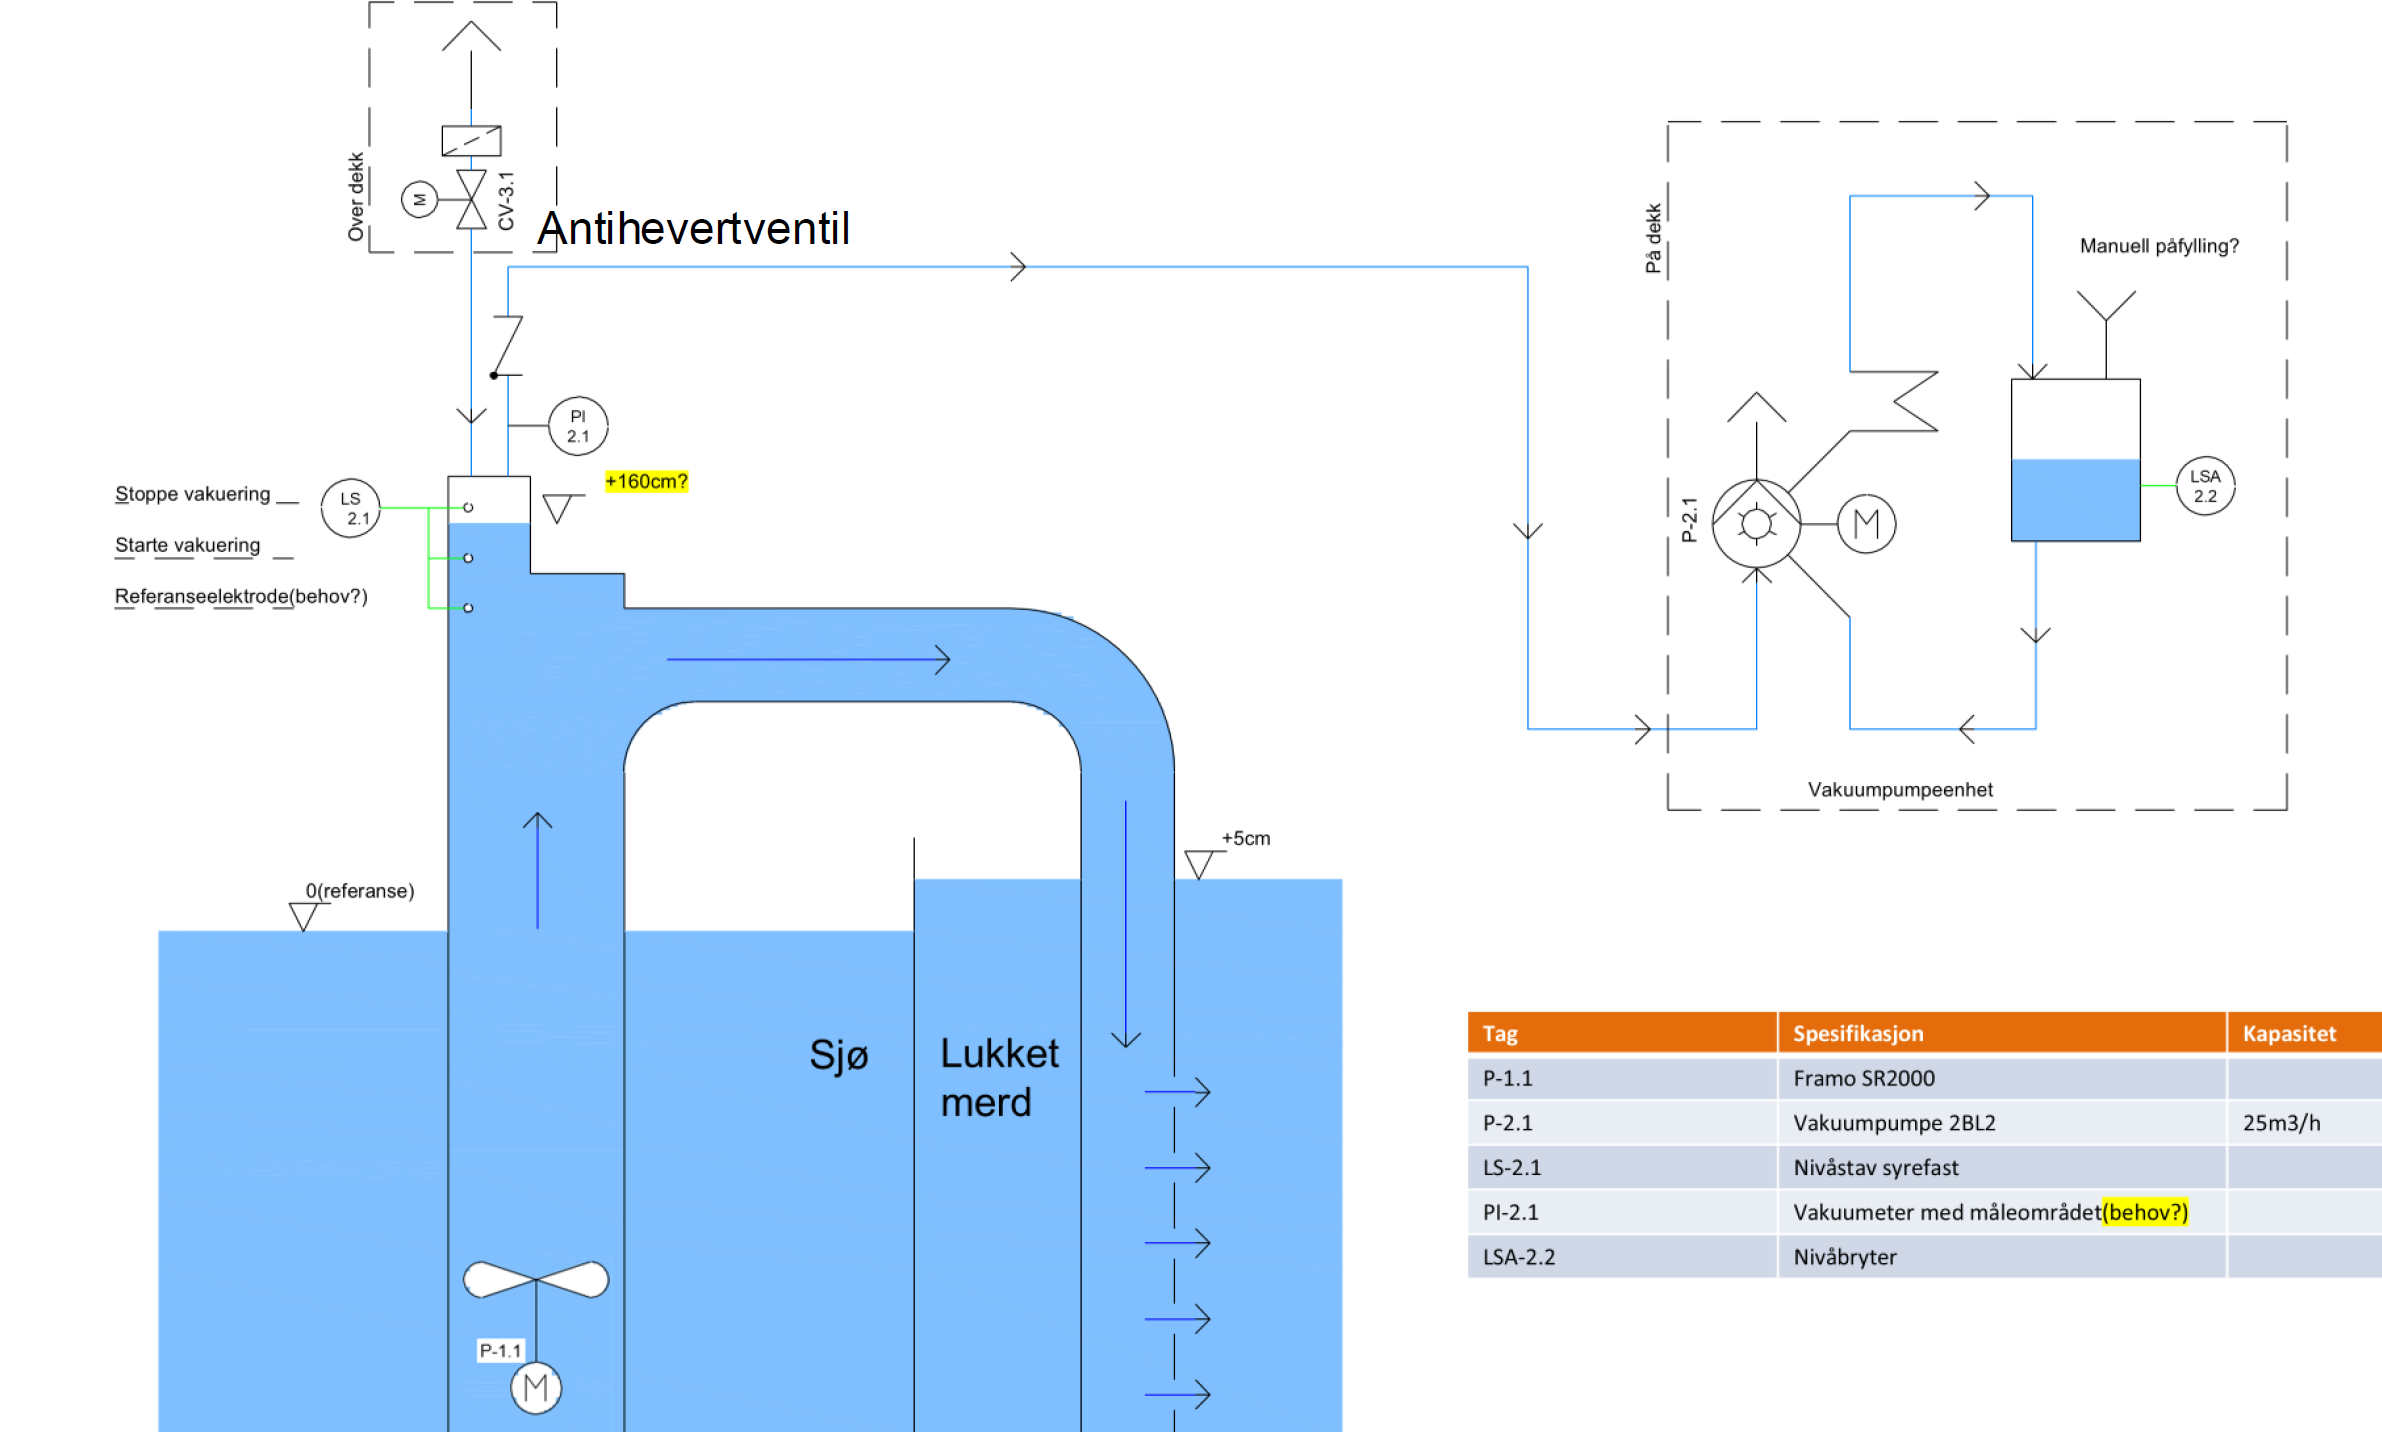
\includegraphics [width=.53\textwidth]{siphon.png} \newline
\framebox{\parbox{\dimexpr\linewidth-2\fboxsep-2\fboxrule}{
\scriptsize \begin{enumerate}
\item<1-> All systems are powered up and outlet valve is in position within valid range.
\item<2-> User sends start command to pump no. 1
\item<3-> System checks condition of process and begins the starting sequence of inlet pump.
\item<4-> The pumps starts at reduced speed, vacuum system starts and anti-siphon valve closes.
\item<5-> Limit switch has not triggered within the defined time.
\item<6-> System changes to "failed to start", stop command is sent to the pump and anti siphon valve opens.
\end{enumerate}
\textbf{Finish}
\vspace{0.1cm}
\hrule
\vspace{0.1cm}
Scenario 2 - Cold start of inlet pump no. 1 into failed to start state.
  }}

\end{frame}

\begin{frame}
\frametitle{Scenarios}
\onslide<4->{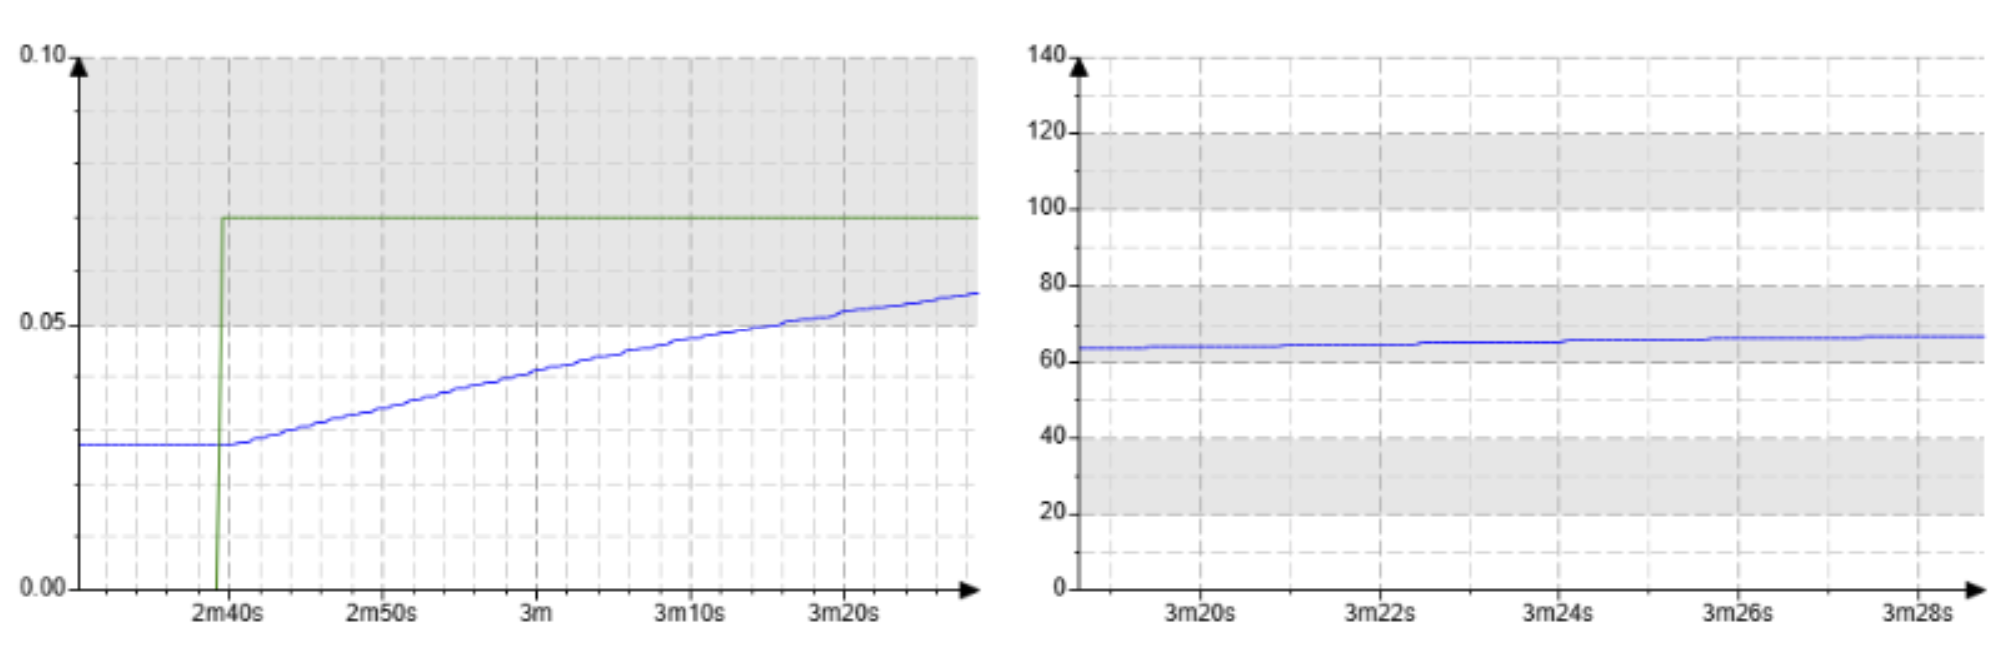
\includegraphics[width=\textwidth]{snip1.png}} \newline
\framebox{\parbox{\dimexpr\linewidth-2\fboxsep-2\fboxrule}{
\footnotesize \begin{enumerate}
\item<1-> All pumps have started and is running in remote operation at 50RPM.
\item<2-> Send auto command to controller.Verify that the controller set point is updated with the current value.
\item<3-> Verify that the RPM control signal to the pumps are stable at around 50RPM.
\item<4-> Change set point to 7cm. Verify that RPM control signal and delta height is stable and rising towards stationary values.
\end{enumerate}
\textbf{Finish}
\vspace{0.1cm}
\hrule
\vspace{0.1cm}
Scenario 3 - Putting the pumps in auto mode after startup and update the set point to the regulator.
  }}

\end{frame}

\begin{frame}
\frametitle{Scenarios}
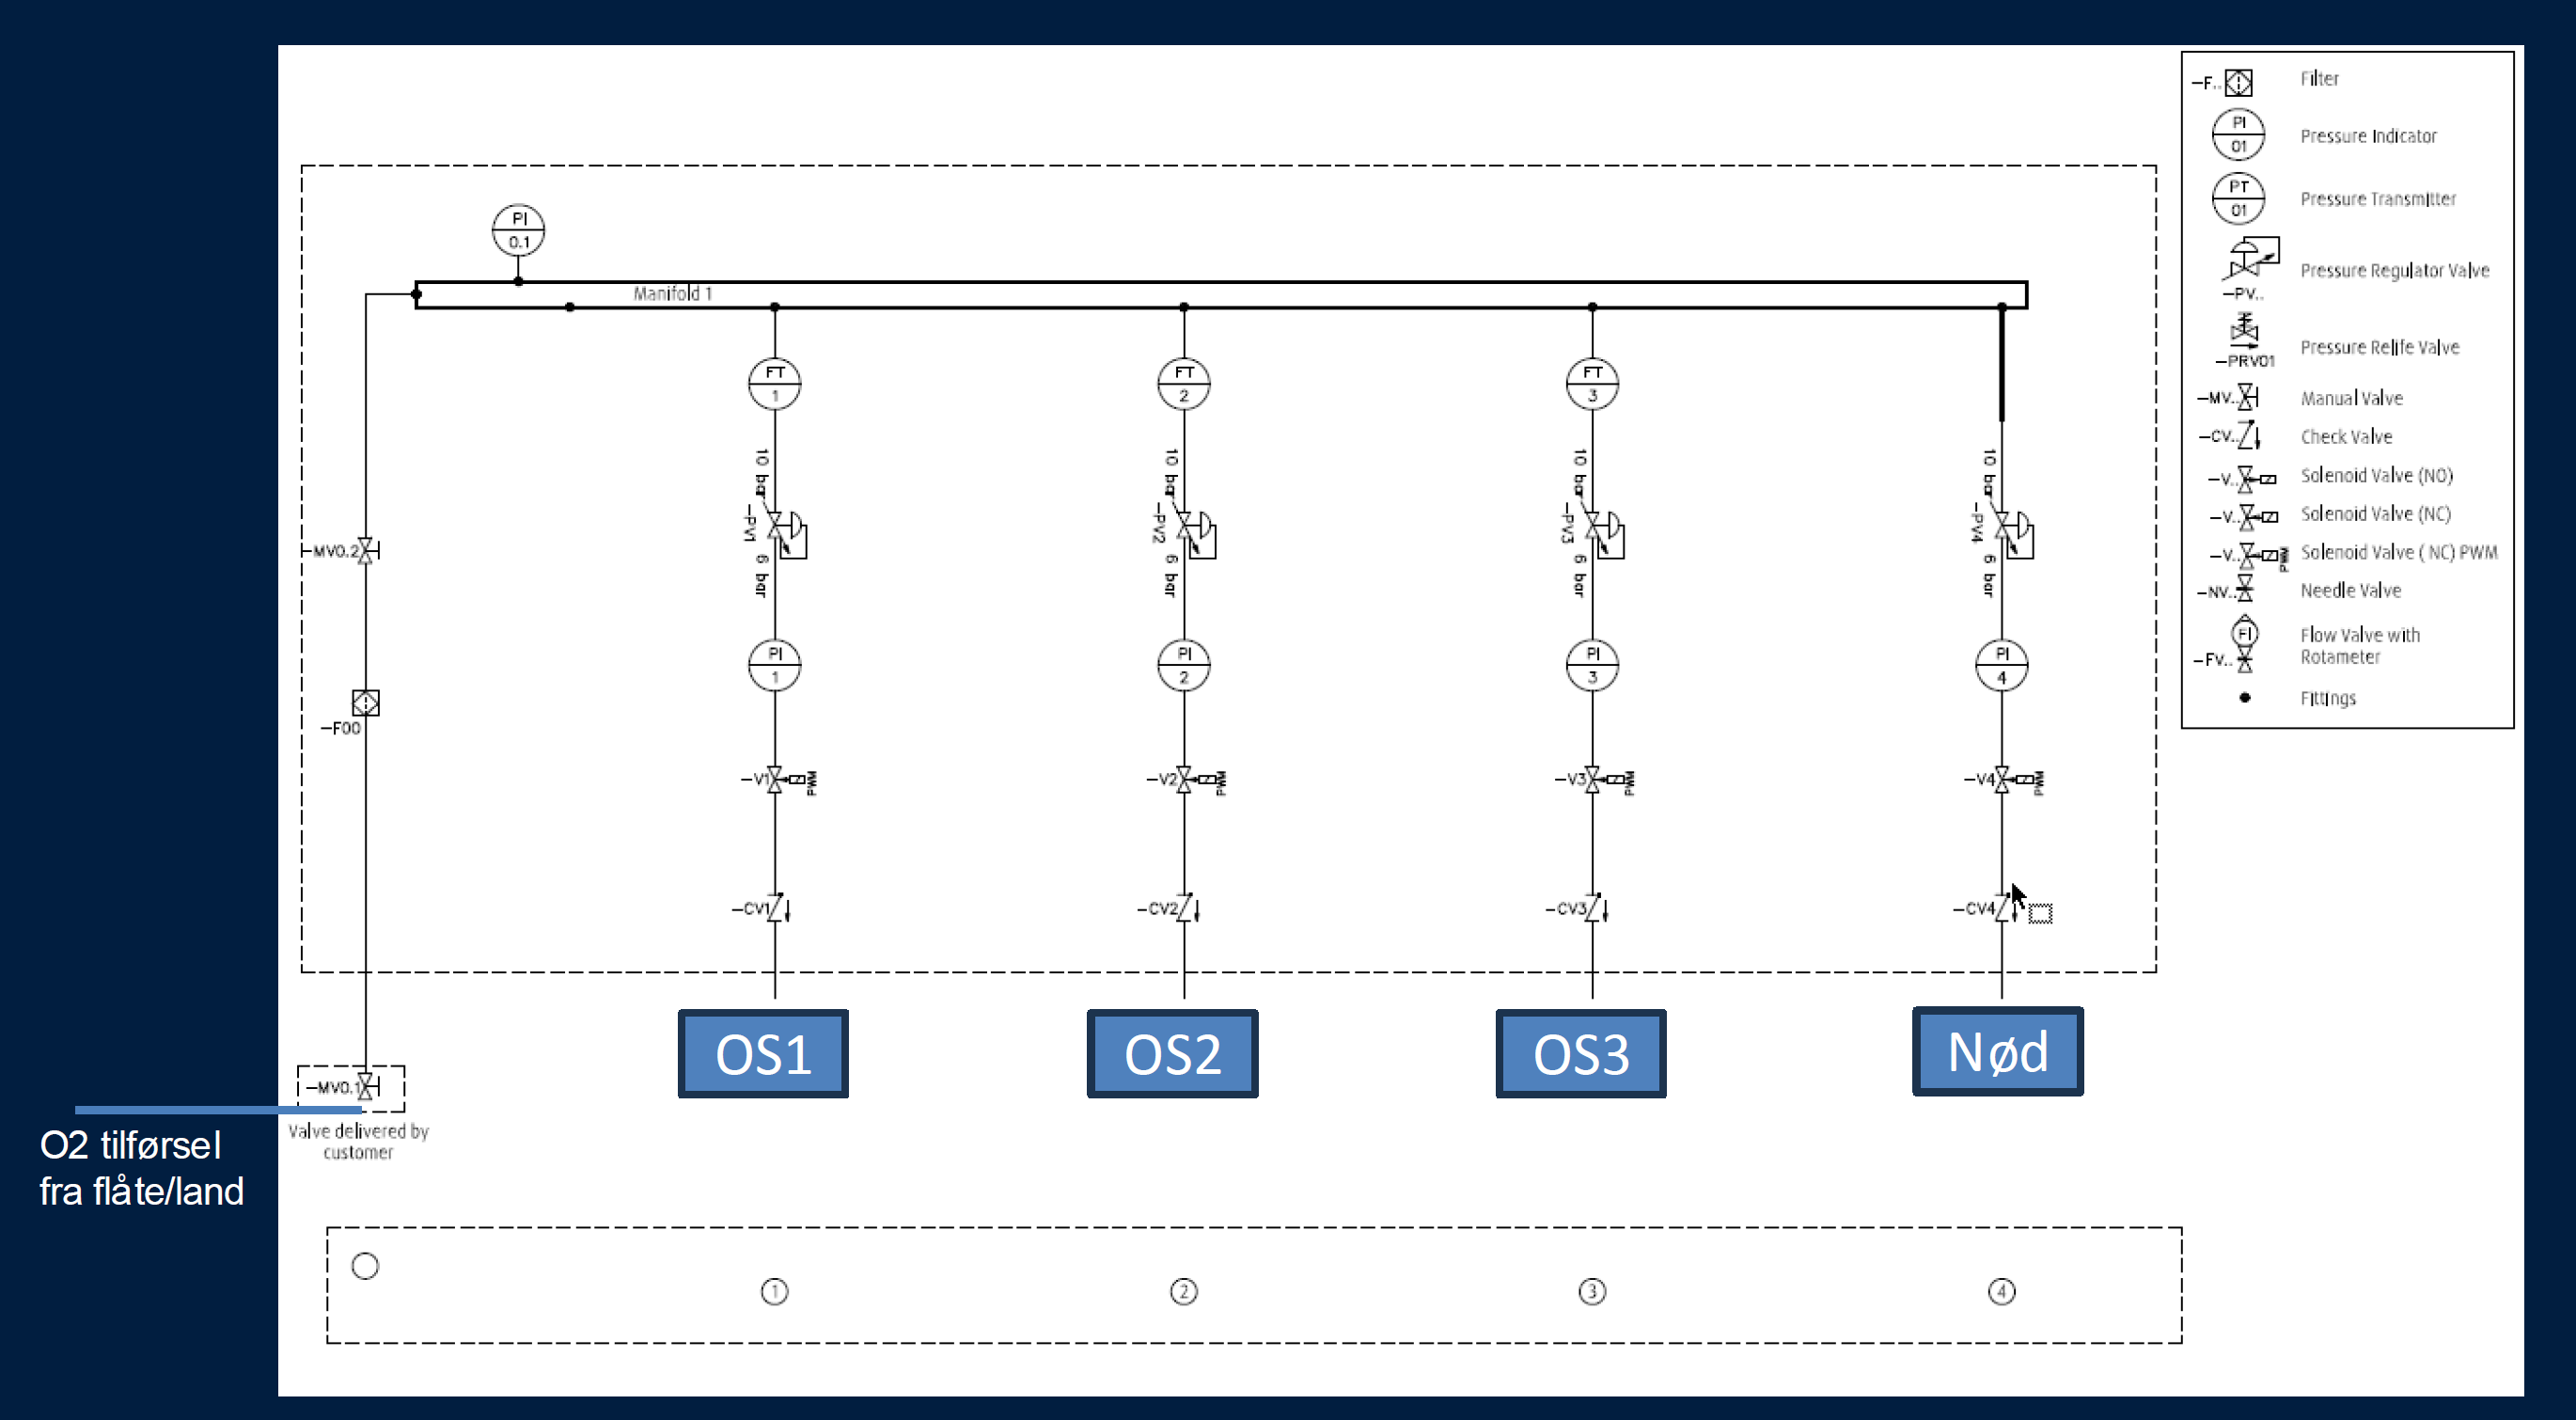
\includegraphics [width=.65\textwidth]{o2_distr_draw.png} \newline
\framebox{\parbox{\dimexpr\linewidth-2\fboxsep-2\fboxrule}{
\footnotesize \begin{enumerate}
\item<1-> Inlet pump no. 1 is running at above minimum speed.
\item<2-> We have minimum pressure at oxygen piping manifold.
\item<3-> Operator sends start signal to the oxygenator system no. 1.
\item<4-> Control valve is set to a manual predefined position.
\item<5-> Solenoid valve opens.
\item<6-> Operator sends "auto mode" signal.
\item<7-> Operator changes set point to the desired oxygen concentration.
\item<8-> Operator verifies that the valve control signal and oxygen concentration levels are stable and moving towards a stationary value.
\end{enumerate}
\textbf{Finish}
\vspace{0.1cm}
\hrule
\vspace{0.1cm}
Scenario 3 - Start oxygenator system from cold start to auto mode
  }}

\end{frame}


\end{document}